% Name: Crystal field splitting
% Description: The five d orbitals of a free metal ion, and how a tetrahedral and an octahedral field split them, with the octahedral gap Δₒ and the tetrahedral gap Δₜ = 4/9 Δₒ about the same mean energy.
% Tags: crystal field theory, d orbitals, octahedral, tetrahedral, splitting

\usetikzlibrary{arrows.meta}

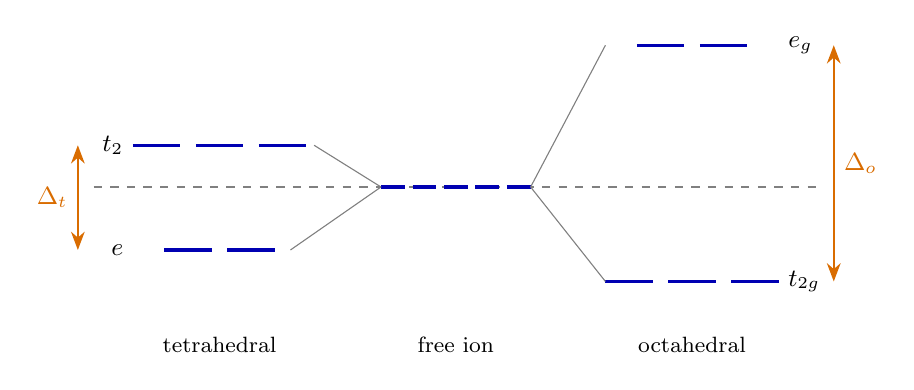
\begin{tikzpicture}[>={Stealth}, every node/.style={font=\small}, lvl/.style={very thick, blue!70!black}]
  % With Δₒ = 3: e_g at +0.6Δₒ = 1.8 and t₂g at -0.4Δₒ = -1.2; Δₜ = 4/3, so t₂ at +0.4Δₜ ≈ 0.53 and e at -0.6Δₜ = -0.8
  \draw[dashed, gray] (-4.6,0) -- (4.6,0);
  \foreach \x in {-0.8,-0.4,0,0.4,0.8} \draw[lvl] (\x-0.15,0) -- (\x+0.15,0);
  \foreach \x in {2.6,3.4} \draw[lvl] (\x-0.3,1.8) -- (\x+0.3,1.8);
  \foreach \x in {2.2,3,3.8} \draw[lvl] (\x-0.3,-1.2) -- (\x+0.3,-1.2);
  \foreach \x in {-3.8,-3,-2.2} \draw[lvl] (\x-0.3,0.53) -- (\x+0.3,0.53);
  \foreach \x in {-3.4,-2.6} \draw[lvl] (\x-0.3,-0.8) -- (\x+0.3,-0.8);
  \draw[gray, thin] (0.95,0) -- (1.9,1.8) (0.95,0) -- (1.9,-1.2) (-0.95,0) -- (-1.8,0.53) (-0.95,0) -- (-2.1,-0.8);
  \node[right] at (4.1,1.8) {$e_g$};
  \node[right] at (4.1,-1.2) {$t_{2g}$};
  \node[left] at (-4.1,0.53) {$t_2$};
  \node[left] at (-4.1,-0.8) {$e$};
  \draw[<->, thick, orange!85!black] (4.8,-1.2) -- node[right] {$\Delta_o$} (4.8,1.8);
  \draw[<->, thick, orange!85!black] (-4.8,-0.8) -- node[left] {$\Delta_t$} (-4.8,0.53);
  \foreach \x/\t in {-3/tetrahedral, 0/free ion, 3/octahedral} \node[font=\footnotesize] at (\x,-2) {\t};
\end{tikzpicture}
